\section{Circular}

\begin{figure}[h]
\centering
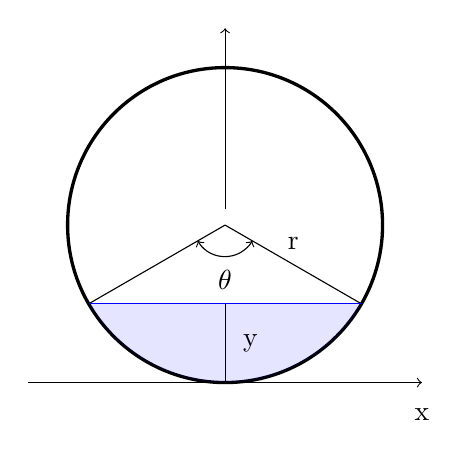
\begin{tikzpicture}
\draw[very thick] (0,0) circle (2);
\draw (0,0)--node[above=2]{r} (1.732051, -1);
\draw (0,0)--(-1.732051, -1);

\draw [<->] (-0.3464, -0.2) arc [radius=0.4, start angle=210, end angle=330];

\node at (0, -0.7) {$\theta$};

\draw[blue] (-1.732051, -1) -- (1.732051, -1);

\filldraw[fill=blue, opacity=0.1](-1.732, -1) arc[x radius=2, y radius = 2, start angle = 210, end angle=330];

\draw (0,-1)--node[right=3]{y} (0,-2);

\draw[->](-2.5,-2) --(2.5, -2) node[below =6]{x} ;
\draw[->](0, 0.2) --(0,2.5);

\end{tikzpicture}
\caption{Circular Section}
\end{figure}

%\subsection{Basic Equations}
\begin{equation}
y = r(1 - \cos\frac{\theta}{2})
\end{equation}

\begin{equation}
A = \frac{1}{2} (\theta - \sin\theta) r^2
\end{equation}

\begin{equation}
P =  \theta r
\end{equation}

\begin{equation}
R = \frac{1}{2} \left(1 - \frac{\sin\theta}{\theta} \right) r
\end{equation}

%\begin{equation}
%T_w = 2r \sin \frac{\theta}{2}
%\end{equation}

\begin{equation}
\frac{\partial y}{\partial \theta} = \frac{r}{2}\sin \frac{\theta}{2}
\end{equation}

\begin{equation}
\frac{\partial A}{\partial \theta} = \frac{1}{2} (1 - \cos\theta) r^2
\end{equation}

\begin{equation}
\frac{\partial A}{\partial y} = \frac{\frac{\partial A}{\partial \theta}}{\frac{\partial y}{\partial \theta}} = \frac{\frac{1}{2} (1 - \cos\theta) r^2}{\frac{r}{2}\sin \frac{\theta}{2}} = 2r\sin\frac{\theta}{2}
\end{equation}

\begin{equation}
\frac{\partial}{\partial \theta}\left(\frac{dA}{dy}\right) = r\cos\frac{\theta}{2} = T_w
\end{equation}

\begin{equation}
\frac{\partial P}{\partial \theta} =  r
\end{equation}

%\begin{equation}
%\frac{dT}{d\theta} = r \cos \frac{\theta}{2}
%\end{equation}

%\subsection{Calculate Maximum Discharge Using Manning's Equation}
%\begin{equation}  
%Q = \frac{K_u}{n}AR^{2/3}S^{1/2} = \frac{K_u}{n}A^{5/3}P^{-2/3}S^{1/2},
%\end{equation}

%\begin{equation}  
%\frac{dQ}{d\theta} = \frac{K_u}{n} \left(\frac{5}{3}R^{2/3}\frac{\partial A}{\partial \theta} -  \frac{2}{3}R^{5/3}\frac{\partial P}{\partial \theta} \right) S^{1/2}=0,
%\end{equation}
%
%\begin{equation}  
%5\frac{\partial A}{\partial \theta} -  2 R\frac{\partial P}{\partial \theta} = 0,
%\label{Eq:CircularMaxQ}
%\end{equation}

\noindent To calculate $\theta_{max}$, $y_{max}$, and $Q_{max}$, Eq. (\ref{Eq:MaxQ}) 
\begin{equation}  
5PA' -  2 AP' = 5\theta r \frac{1}{2} (1 - \cos\theta) r^2 - 2 \frac{1}{2} (\theta - \sin\theta) r^2 r =   3\theta - 5\theta \cos \theta + 2 \sin \theta = 0,
\end{equation}
i.e.,
\begin{equation}  
 3\theta - 5\theta \cos \theta + 2 \sin \theta = 0,
\end{equation}
The $\theta$ when $Q$ peaks,
\begin{equation}  
\theta_{max}  = 5.27810713,
\end{equation}

\begin{equation}  
Q_{max} =  2.2189 \frac{K_u}{n} r^{8/3}S^{1/2},
\end{equation}

\begin{equation}  
y_{max}  = 1.87636243 r.
\end{equation}

\noindent Neton's method is used to calculate normal depth $y_n$ and critical depth $y_c$.
%\subsection{Calculate Normal Depth}
%For $Q$ less than $Q_{max}$,
%\begin{equation}  
%\theta_{i+1} = \theta_i -\frac{f_d(\theta_{i})}{f'_d(\theta_{i})}
%\end{equation}
%where
%\begin{equation}  
%f_d(\theta_{i})= \frac{K_u}{n}A^{5/3}P^{-2/3}S^{1/2} - Q 
%\end{equation}

%\begin{equation}  
%f'_d(\theta_{i})= \frac{K_u}{n}\left(\frac{5}{3}R^{2/3}\frac{\partial A}{\partial \theta} -  \frac{2}{3}R^{5/3}\frac{\partial P}{\partial \theta}\right)S^{1/2}
%\end{equation}

%\subsection{Calculate Critical Depth}

%\begin{equation}  
%\frac{\partial A}{\partial y} (\theta)= \frac{\frac{\partial A}{\partial \theta}}{\frac{\partial y}{\partial \theta}}=\frac{1-\cos\theta}{\sin \theta/2}r = 2r\sin\frac{\theta}{2}
%\end{equation}

%\begin{equation}  
%\frac{\partial}{\partial \theta} \left(\frac{\partial A}{\partial y} \right) = r \cos \frac{\theta}{2}
%\end{equation}


%\begin{equation}  
%f_c(\theta)= gA^3 - Q^2\frac{\partial A}{\partial y} =  gA^3 - 2rQ^2 \sin\frac{\theta}{2}
%\end{equation}

%\begin{equation}  
%f'_c(\theta)= 3gA^2\frac{\partial A}{\partial \theta} - Q^2\frac{\partial}{\partial \theta} \left(\frac{\partial A}{\partial y} \right)
%\end{equation}
